\documentclass[a4paper,11pt,fleqn,dvipsnames,oneside,openright]{memoir} 	%
% Openright aabner kapitler paa hoejresider (openany begge)
%\newcommand*{\docroot}{.}%Sætter relativ rod af dokumentet
% ¤¤ Oversaettelse og tegnsaetning ¤¤ %
\usepackage[utf8]{inputenc}					% Input-indkodning af tegnsaet (UTF8)
\usepackage[danish]{babel}					% Dokumentets sprog
\usepackage[T1]{fontenc}					% Output-indkodning af tegnsaet (T1)
\usepackage{ragged2e,anyfontsize}			% Justering af elementer
%\usepackage{fixltx2e}						% Retter forskellige fejl i LaTeX-kernen

\usepackage{lmodern}

\usepackage{datetime} % Nuværende tidspunkt

% ¤¤ Figurer og tabeller (floats) ¤¤ %
\usepackage{graphicx} 						% Haandtering af eksterne billeder (JPG, PNG, EPS, PDF)s
%\usepackage{eso-pic}						% Tilfoej billedekommandoer paa hver side
\usepackage{wrapfig}						% Indsaettelse af figurer omsvoebt af tekst. \begin{wrapfigure}{Placering}{Stoerrelse}
%\usepackage{subcaption}					% Included i memoir class

\usepackage{multirow}                		% Fletning af raekker og kolonner (\multicolumn og \multirow)
\usepackage{multicol}         	        	% Muliggoer output i spalter
\usepackage{rotating}						% Rotation af tekst med \begin{sideways}...\end{sideways}
\usepackage{colortbl} 						% Farver i tabeller (fx \columncolor og \rowcolor)
\usepackage{xcolor}							% Definer farver med \definecolor. Se mere: http://en.wikibooks.org/wiki/LaTeX/Colors
\usepackage{flafter}						% Soerger for at floats ikke optraeder i teksten foer deres reference
\let\newfloat\relax 						% Justering mellem float-pakken og memoir
\usepackage{float}							% Muliggoer eksakt placering af floats, f.eks. \begin{figure}[H]
\usepackage{longtable} %Long tables

\usepackage{afterpage} %Bruges til at få billeder og figurer til at være samen med kapitlet de hører til
\usepackage{placeins}

% ¤¤ Matematik mm. ¤¤
\usepackage{amsmath,amssymb,stmaryrd} 		% Avancerede matematik-udvidelser
\usepackage{mathtools}						% Andre matematik- og tegnudvidelser
\usepackage{textcomp}                 		% Symbol-udvidelser (f.eks. promille-tegn med \textperthousand )
\usepackage{rsphrase}						% Kemi-pakke til RS-saetninger, f.eks. \rsphrase{R1}
\usepackage[version=3]{mhchem} 				% Kemi-pakke til flot og let notation af formler, f.eks. \ce{Fe2O3}
\usepackage{siunitx}						% Flot og konsistent praesentation af tal og enheder med \si{enhed} og \SI{tal}{enhed}
\sisetup{locale=DE}							% Opsaetning af \SI (DE for komma som decimalseparator) 

% ¤¤ Referencer og kilder ¤¤ %
\usepackage[danish]{varioref}				% Muliggoer bl.a. krydshenvisninger med sidetal (\vref)
%\usepackage{natbib}							% Udvidelse med naturvidenskabelige citationsmodeller
%\usepackage{xr}							% Referencer til eksternt dokument med \externaldocument{<NAVN>}
%\usepackage{glossaries}					% Terminologi- eller symbolliste (se mere i Daleifs Latex-bog)

% ¤¤ Misc. ¤¤ %
\usepackage{lipsum}							% Dummy text \lipsum[..]
\usepackage[shortlabels]{enumitem}			% Muliggoer enkelt konfiguration af lister
\usepackage{pdfpages}						% Goer det muligt at inkludere pdf-dokumenter med kommandoen \includepdf[pages={x-y}]{fil.pdf}

%EMF to PDF conversion
\usepackage{epstopdf}

% Kommentarer og rettelser med \fxnote. Med 'final' i stedet for 'draft' udloeser hver note en error i den faerdige rapport.
\usepackage[footnote,danish,final,nomargin]{fixme}

% Microtype gør at teksten ser pænere ud.
\usepackage{microtype}

\usepackage{listings}
\usepackage{titlesec}
%Usecase and accepttest numbering
%% Se http://en.wikibooks.org/wiki/LaTeX/Counters http://en.wikibooks.org/wiki/LaTeX/Labels_and_Cross-referencing og http://en.wikibooks.org/wiki/LaTeX/Macros for info på hvordan nedenståen er opstået

\newcounter{usecases} %counter
\newcommand{\usecaseset}[1]{\#\refstepcounter{usecases}\arabic{usecases}\label{usecase:#1}} %Tacking an usecase
\newcommand{\usecaseref}[1]{\ref{usecase:#1}} %referencing a usecase

\newcounter{accepttests} %counter
\newcommand{\accepttestset}[1]{\#\refstepcounter{accepttests}\arabic{accepttests}\label{accepttest:#1}}
\newcommand{\accepttestref}[1]{\ref{accepttest:#1}}

%Inkludering af class diagram
\newcommand{\includeclassdiagram}[2]{\includegraphics[width=#1,clip=true,trim=39
40 39 40]{#2}}

%Ens navne på x10 enheder
\newcommand{\xti}{X10}
\newcommand{\xtic}{X10-controller}
\newcommand{\xtie}{X10-enhed}
\newcommand{\xtis}{X10-slave}

\newsubfloat{figure}

%%%% CUSTOM SETTINGS %%%%

\pdfoptionpdfminorversion=6					% Muliggoer inkludering af pdf dokumenter, af version 1.6 og hoejere
\pretolerance=2500 							% Justering af afstand mellem ord (hoejt tal, mindre orddeling og mere luft mellem ord)

% ¤¤ Marginer ¤¤ %
\setlrmarginsandblock{3.5cm}{2.5cm}{*}		% \setlrmarginsandblock{Indbinding}{Kant}{Ratio}
\setulmarginsandblock{2.5cm}{3.0cm}{*}		% \setulmarginsandblock{Top}{Bund}{Ratio}
\checkandfixthelayout 						% Oversaetter vaerdier til brug for andre pakker

%	¤¤ Afsnitsformatering ¤¤ %
\setlength{\parindent}{0mm}           		% Stoerrelse af indryk
\setlength{\parskip}{3mm}          			% Afstand mellem afsnit ved brug af double Enter
\linespread{1,1}							% Linie afstand

% ¤¤ Litteraturlisten ¤¤ %
%\bibpunct[,]{[}{]}{;}{a}{,}{,} 				% Definerer de 6 parametre ved Harvard
% henvisning (bl.a. parantestype og seperatortegn) \bibliographystyle{bibtex/harvard}			% Udseende af litteraturlisten.
\bibliographystyle{plain}			% Udseende af litteraturlisten.

% ¤¤ Indholdsfortegnelse ¤¤ %
\setsecnumdepth{subsection}		 			% Dybden af nummerede overkrifter (part/chapter/section/subsection)
\maxsecnumdepth{subsection}					% Dokumentklassens graense for nummereringsdybde
\settocdepth{subsection} 					% Dybden af indholdsfortegnelsen

% ¤¤ Lister ¤¤ %
\setlist{
  topsep=0pt,								% Vertikal afstand mellem tekst og listen
  itemsep=-1ex,								% Vertikal afstand mellem items
} 

% ¤¤ Visuelle referencer ¤¤ %
\usepackage[colorlinks]{hyperref}			% Danner klikbare referencer (hyperlinks) i dokumentet.
\hypersetup{colorlinks = true,				% Opsaetning af farvede hyperlinks (interne links, citeringer og URL)
    linkcolor = black,
    citecolor = black,
    urlcolor = black
}

% % Sprog opsætning for referencer
\def\figureautorefname{Figur}
\def\tableautorefname{Tabel}

% ¤¤ Opsaetning af figur- og tabeltekst ¤¤ %
\captionnamefont{\small\bfseries\itshape}	% Opsaetning af tekstdelen ('Figur' eller 'Tabel')
\captiontitlefont{\small}					% Opsaetning af nummerering
\captiondelim{. }							% Seperator mellem nummerering og figurtekst
\hangcaption								% Venstrejusterer flere-liniers figurtekst under hinanden
\captionwidth{\linewidth}					% Bredden af figurteksten
\setlength{\belowcaptionskip}{10pt}			% Afstand under figurteksten
		
% ¤¤ Navngivning ¤¤ %
\addto\captionsdanish{
	\renewcommand\appendixname{Appendiks}
	\renewcommand\contentsname{Indholdsfortegnelse}	
	\renewcommand\appendixpagename{Appendiks}
	\renewcommand\appendixtocname{Appendiks}
	\renewcommand\cftchaptername{\chaptername~}				% Skriver "Kapitel" foran kapitlerne i indholdsfortegnelsen
	\renewcommand\cftappendixname{\appendixname~}			% Skriver "Appendiks" foran appendiks i indholdsfortegnelsen
}

% ¤¤ Kapiteludssende ¤¤ %
\definecolor{numbercolor}{gray}{0.7}		% Definerer en farve til brug til kapiteludseende
\newif\ifchapternonum

\makechapterstyle{jenor}{					% Definerer kapiteludseende frem til ...
  \renewcommand\beforechapskip{0pt}
  \renewcommand\printchaptername{}
  \renewcommand\printchapternum{}
  \renewcommand\printchapternonum{\chapternonumtrue}
  \renewcommand\chaptitlefont{\fontfamily{pbk}\fontseries{db}\fontshape{n}\fontsize{25}{35}\selectfont\raggedleft}
  \renewcommand\chapnumfont{\fontfamily{pbk}\fontseries{m}\fontshape{n}\fontsize{1in}{0in}\selectfont\color{numbercolor}}
  \renewcommand\printchaptertitle[1]{%
    \noindent
    \ifchapternonum
    \begin{tabularx}{\textwidth}{X}
    {\let\\\newline\chaptitlefont ##1\par} 
    \end{tabularx}
    \par\vskip-2.5mm\hrule
    \else
    \begin{tabularx}{\textwidth}{Xl}
    {\parbox[b]{\linewidth}{\chaptitlefont ##1}} & \raisebox{-15pt}{\chapnumfont \thechapter}
    \end{tabularx}
    \par\vskip2mm\hrule
    \fi
  }
}											% ... her

\chapterstyle{jenor}						% Valg af kapiteludseende - Google 'memoir chapter styles' for alternativer

% ¤¤ Sidehoved ¤¤ %

\makepagestyle{AAU}							% Definerer sidehoved og sidefod udseende frem til ...
\makepsmarks{AAU}{%
	\createmark{chapter}{left}{shownumber}{}{. \ }
	\createmark{section}{right}{shownumber}{}{. \ }
	\createplainmark{toc}{both}{\contentsname}
	\createplainmark{lof}{both}{\listfigurename}
	\createplainmark{lot}{both}{\listtablename}
	\createplainmark{bib}{both}{\bibname}
	\createplainmark{index}{both}{\indexname}
	\createplainmark{glossary}{both}{\glossaryname}
}
\nouppercaseheads											% Ingen Caps oenskes

\makeevenhead{AAU}{Aarhus Universitet - Gruppe 08}{}{\leftmark}				% Definerer lige siders sidehoved (\makeevenhead{Navn}{Venstre}{Center}{Hoejre})
\makeoddhead{AAU}{\rightmark}{}{Gruppe 08 - Aarhus Universitet}		% Definerer ulige siders sidehoved (\makeoddhead{Navn}{Venstre}{Center}{Hoejre})
\makeevenfoot{AAU}{\thepage}{}{}							% Definerer lige siders sidefod (\makeevenfoot{Navn}{Venstre}{Center}{Hoejre})
\makeoddfoot{AAU}{}{}{\thepage}								% Definerer ulige siders sidefod (\makeoddfoot{Navn}{Venstre}{Center}{Hoejre})
\makeheadrule{AAU}{\textwidth}{0.5pt}						% Tilfoejer en streg under sidehovedets indhold
\makefootrule{AAU}{\textwidth}{0.5pt}{1mm}					% Tilfoejer en streg under sidefodens indhold

\copypagestyle{AAUchap}{AAU}								% Sidehoved for kapitelsider defineres som standardsider, men med blank sidehoved
\makeoddhead{AAUchap}{}{}{}
\makeevenhead{AAUchap}{}{}{}
\makeheadrule{AAUchap}{\textwidth}{0pt}
\aliaspagestyle{chapter}{AAUchap}							% Den ny style vaelges til at gaelde for chapters
															% ... her
															
\pagestyle{AAU}												% Valg af sidehoved og sidefod


%%%% CUSTOM COMMANDS %%%%

% ¤¤ Billede hack ¤¤ %
\newcommand{\figur}[4]{
		\begin{figure}[H] \centering
			\includegraphics[width=#1\textwidth]{billeder/#2}
			\caption{#3}\label{#4}
		\end{figure} 
}

% ¤¤ Specielle tegn ¤¤ %
\newcommand{\grader}{^{\circ}\text{C}}
\newcommand{\gr}{^{\circ}}
\newcommand{\g}{\cdot}


%%%% ORDDELING %%%%

\hyphenation{}

% % listings setup
\lstset{
tabsize=4,
frame=single,
columns=fullflexible,
linewidth=\textwidth
}

% % % sørg for at floats er på siden inden en ny section starter
%\newcommand{\sectionbreak}{\clearpage}
%\newcommand{\subsectionbreak}{\FloatBarrier}

%Code handling - Colors lstlisting

\lstset{language=C++,
                basicstyle=\ttfamily,
                keywordstyle=\color{blue}\ttfamily,
                stringstyle=\color{red}\ttfamily,
                commentstyle=\color{green}\ttfamily,
                morecomment=[l][\color{magenta}]{\#}
}


\title{Projektdokumentation}
\author{E3PRJ3 Gruppe ??}
\date{\today{} \currenttime{}}

\begin{document}
% % % Indexes % % %
%\maketitle

\frontmatter
\thispagestyle{empty}
\begin{flushright}
\vspace{2cm}


\textit{\textbf{\textsc{\HUGE Projektdokumentation 3. semester}} \\ \vspace{1cm}}

\rule{13cm}{3mm} \\ \vspace{1cm}

%\includegraphics[width=0.9\textwidth]{billeder/forside.jpg}
\vspace{1cm} 
\textsc{\Large E3PRJ3 \\
Gruppe 8 \\
IKT, Elektro \& Stærkstrøm\\
Aarhus School of Engineering\\
\vspace{0.2cm}
\date{\today{} \currenttime{}}
}
\end{flushright}


\vspace{6.5cm}


\textsc{\Large
\begin{tabular}[\widthof{Studienummer - NavnMMMMM}]{rcl}
\textbf{Studienummer} & \textbf{-} & \textbf{Navn} \\ 
20104209 & - & Andreas Laursen \\
201270024 & - & Dannie Lehmann \\
10253 & - & Jens Rix Jørgensen \\
201270725 & - & Mathias Jessen \\
20062548 & - & Morten Møller Christensen \\
201303580 & - & Simon Mouridsen \\
201270943 & - & Stine Skaarup Høgsberg \\
\\
Vejleder & - & Lars G. Johansen
\end{tabular}
}
\clearpage
\chapter*{Deltageres underskrift}

\phantom{Luft}

\phantom{Luft}

\begin{table}[H]
	\centering
		\begin{tabular}{c c c}
		&&\\
		&&\\
		&&\\
		&&\\
			\underline{\phantom{mmmmmmmmmmmmmm}} && \underline{\phantom{mmmmmmmmmmmmmm}} \\
			Andreas Laursen && Dannie Lehmann\\
			20104209 && 201270024\\
			&&\\
			&&\\
			&&\\
			&&\\
			&&\\
			\underline{\phantom{mmmmmmmmmmmmmm}} && \underline{\phantom{mmmmmmmmmmmmmm}} \\
			Jens Rix Jørgensen && Mathias Jessen\\
			10253 && 201270725\\
			&&\\
			&&\\
			&&\\
			&&\\
			&&\\
			\underline{\phantom{mmmmmmmmmmmmmm}} && \underline{\phantom{mmmmmmmmmmmmmm}} \\
			Morten Møller Christensen && Simon Mouridsen\\
			20062548 && 201303580\\
			&&\\
			&&\\
			&&\\
			&&\\
			&&\\
		 							& \underline{\phantom{mmmmmmmmmmmmmm}} 	&			\\														
									& Stine Skaarup Høgsberg\\
									& 201270943								
		\end{tabular}
\end{table}


%indholdsfortegnelse
\clearpage
\tableofcontents*

\mainmatter
\chapter{Kravspecifikation}

\section{Use Case diagram}

\begin{figure}[h]
\centering
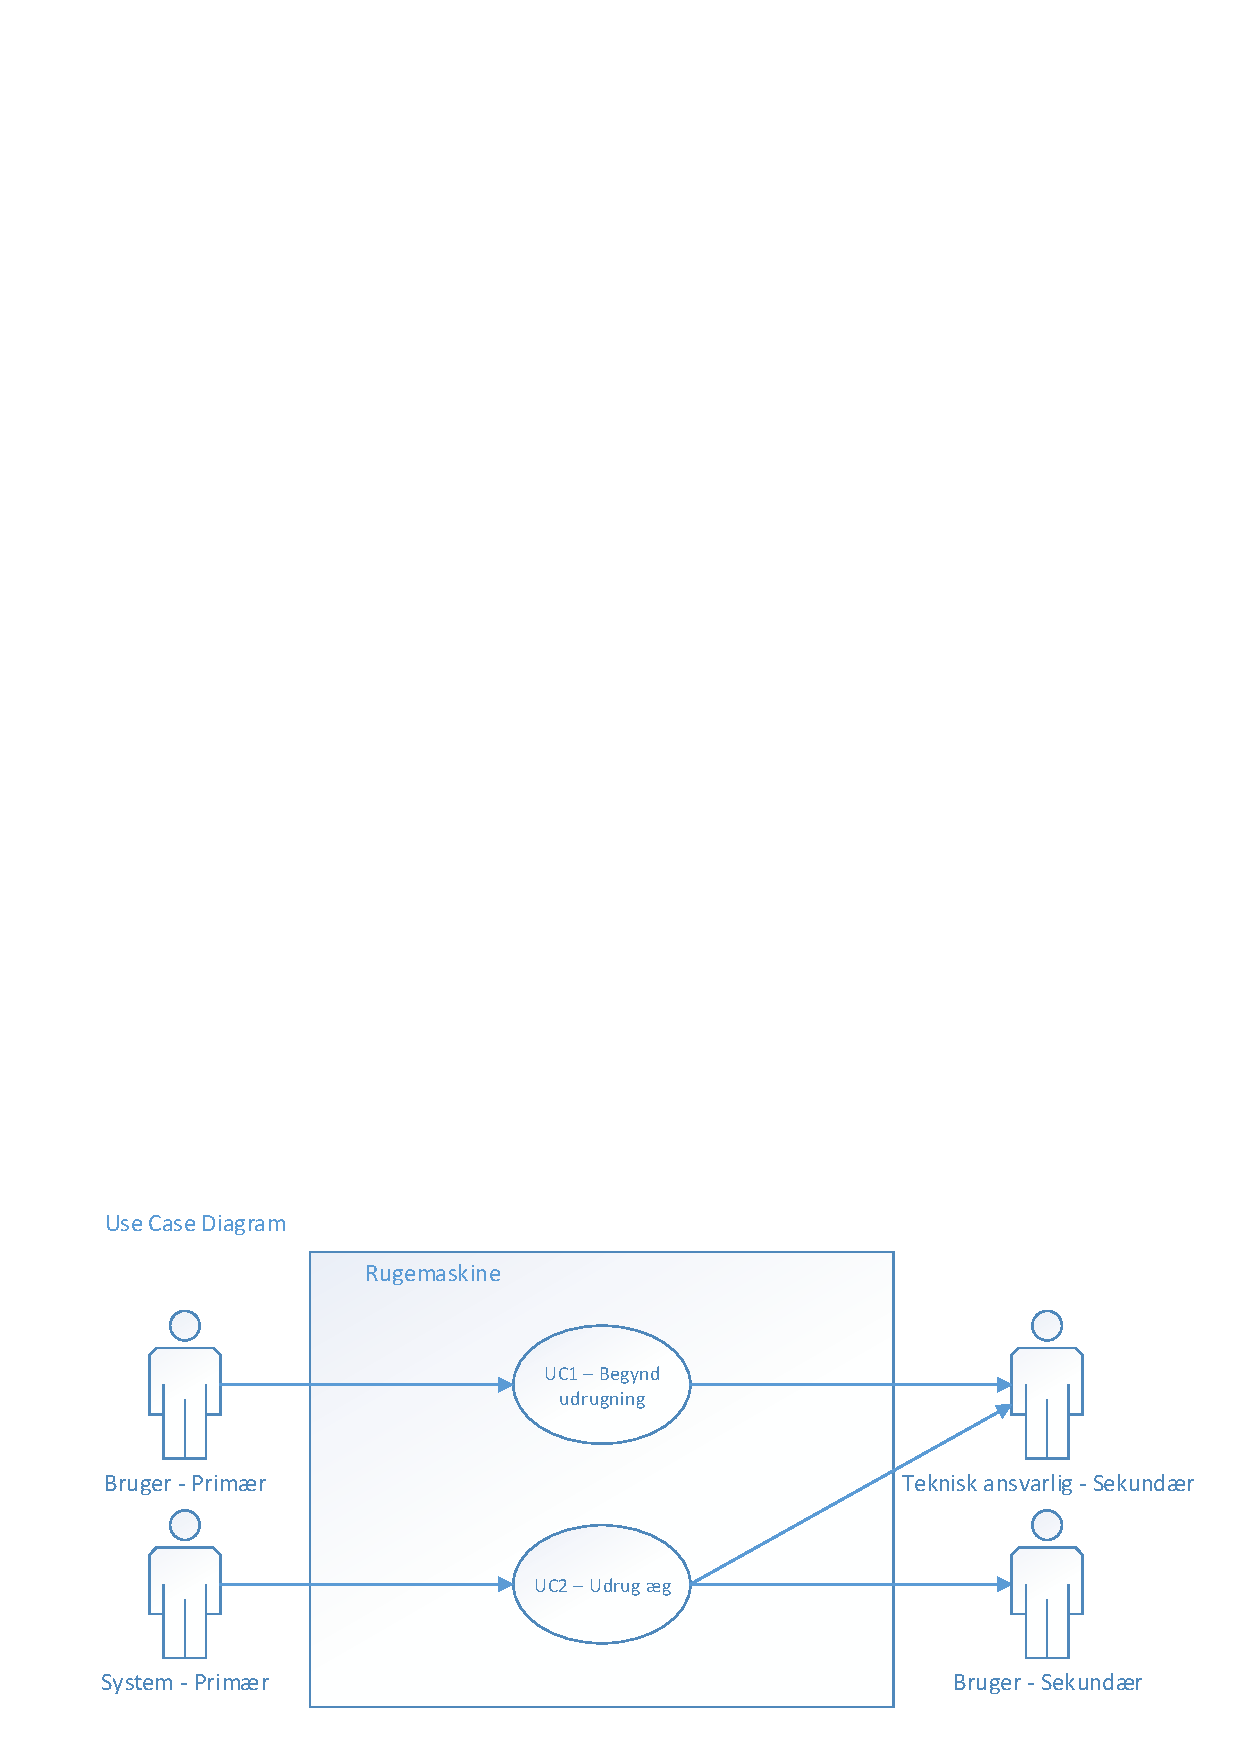
\includegraphics[width=16cm, scale=1, trim= 0mm 0mm 0mm 200mm, clip=true,  angle=0]{1_kravspecifikation/diagrammer/UseCase_Generel_v1.pdf}
\caption{Use Case diagram}
\label{fig:usecase_diagram}
\end{figure}

\clearpage
\section{Aktørbeskrivelse}

\subsection{Bruger}

\begin{table}[H]
\centering
\begin{tabular}[\textwidth]{|p{0.20\textwidth}|p{0.80\textwidth}|}
\hline Aktørnavn: & Bruger \\ 
\hline Alternativt navn: & User \\ 
\hline Type: & Primær og sekundær\\ 
\hline Beskrivelse: & 
		\begin{enumerate}
		\item Bruger ønsker at udruge æg
		\end{enumerate} \\ 
\hline
\end{tabular}
\caption{Aktør - Bruger}
\label{tab:usecase-aktoer-bruger}
\end{table}



\subsection{System}

\begin{table}[H]
\centering
\begin{tabular}[\textwidth]{|p{0.20\textwidth}|p{0.80\textwidth}|}
\hline Aktørnavn: & System \\ 
\hline Alternativt navn: & Rugemaskine \\ 
\hline Type: & Primær \\ 
\hline Beskrivelse: & 
		\begin{enumerate}
		\item Systemet styrer udrugningsprocesser.
		\item Systemet har til opgave at overvåge temperatur, luftfugtighed samt tidsprogression.
		\end{enumerate} \\ 
\hline
\end{tabular}
\caption{Aktør - System}
\label{tab:usecase-aktoer-system}
\end{table}



\subsection{Tekniske ansvarlig}

\begin{table}[H]
\centering
\begin{tabular}[\textwidth]{|p{0.20\textwidth}|p{0.80\textwidth}|}
\hline Aktørnavn: & Tekniske ansvarlig \\ 
\hline Alternativt navn: & Servicetekniker \\ 
\hline Type: & Ekstern \\ 
\hline Beskrivelse: & 
		\begin{enumerate}
		\item Tekniske ansvarlig er en uddannet tekniker, der har en faglig forståelse for opbygning af rugemaskinen.
		\end{enumerate} \\ 
\hline
\end{tabular}
\caption{Aktør - Tekniske ansvarlig}
\label{tab:usecase-aktoer-tekniskeansvarlig}
\end{table}


\clearpage

\section{Use Cases}
\subsection{Begynd udrugning}

\begin{table}[H]
\centering
\begin{tabular}[\textwidth]{|p{0.18\textwidth}|p{0.82\textwidth}|}
\hline Navn & Begynd udrugning \\ 
\hline Usecase ID & \usecaseset{Begynd udrugning} \\ 
\hline Scope &  \\
\hline Primær aktør & Bruger \\ 
\hline Interessenter & Tekniske ansvarlig. \\ 
\hline Forudsætning & Use Case \usecaseref{Udrug aeg} er ikke aktiv \\ 
\hline Resultat & Udrugning af indlagte æg er påbegyndt. \\ 
\hline Hovedforløb &
	\begin{enumerate}
	\item \label{itm:Begynd-step1} Bruger åbner låge.
	\item \label{itm:Begynd-step2} Systemet registrerer åbning af låge. 
	\item \label{itm:Begynd-step3} Systemet låser for interfacet (skriver "låge åben").
	\item \label{itm:Begynd-step4} Bruger placerer æg i maskine.
	\item \label{itm:Begynd-step5} Bruger lukker låge.
	\item \label{itm:Begynd-step6} Systemet registrerer lukning af låge.  
	\item \label{itm:Begynd-step7} Systemet låser op for interfacet (fjerner "låge åben").
	\item \label{itm:Begynd-step8} Bruger vælger type af æg til udrugning (sekvens).
	\item \label{itm:Begynd-step9} Systemet spørger bruger om bekræftelse.
	\item \label{itm:Begynd-step10} Bruger bekræfter valg (vælger "OK").
	\item \label{itm:Begynd-step11} Systemet registrerer valg.
	\item \label{itm:Begynd-step12} Systemet aktiverer sekvensen Udrug Æg (Use Case \usecaseref{Udrug aeg}).
%	\item \label{itm:Begynd-step12} 
	\end{enumerate} \\
	\hline Undtagelser &
	\begin{enumerate}
	\item[\ref{itm:Begynd-step2}a.] System registrerer ikke åbning af låge. 
	\begin{itemize}
	\item Bruger kontakter teknisk ansvarlig. 
	\end{itemize}
	\item[\ref{itm:Begynd-step6}a.] System registrerer ikke lukning af låge.  
	\begin{itemize}
	\item Bruger kontakter teknisk ansvarlig. 
	\end{itemize}
	\item[\ref{itm:Begynd-step10}a.] Bruger bekræfter ikke valg (vælger "Annullér"). 
	\begin{itemize}
	\item Step \ref{itm:Begynd-step8} gentages.
	\end{itemize}
	\end{enumerate} \\
\hline 
\end{tabular}
\caption{Use Case - Begynd udrugning}
\label{tab:usecase-Begynd-udrugning}
\end{table}
\linespread{1.0}\subsection{Udrug {\ae}g}
\begin{table}[H]
\centering
\begin{tabular}[\textwidth]{|p{0.18\textwidth}|p{0.82\textwidth}|}
\hline Navn & Udrug æg \\ 
\hline Usecase ID & \usecaseset{Udrug aeg} \\ 
\hline Primær aktør & System \\ 
\hline Interessenter & Sekundær aktør: Bruger \\ 
\hline Forudsætning & Use Case \usecaseref{Begynd udrugning} \\ 
\hline Resultat & Æggene er udruget og fjernet fra maskinen \\ 
\hline Hovedforløb &
	\begin{enumerate}
	\item \label{itm:udrugning-step1} Systemet indlæser valgte sekvens.
	\item \label{itm:udrugning-step2} Systemet regulerer temperatur og luftfugtighed.
	\item \label{itm:udrugning-step3} Systemet kontrollerer om det er tid til æggevending.  \newline
	\textbf{hvis} (tid = æggevending): Vend æg.
	\newline
	\textbf{ellers}: Vend ikke æg.
	\newline
	Step \ref{itm:udrugning-step2}-\ref{itm:udrugning-step3} gentages indtil udrugningstiden er afsluttet.
	\item \label{itm:udrugning-step4} 	System informerer brugeren om at udrugningssekvens er færdig.
	\item \label{itm:udrugning-step5} 	Bruger åbner låge.
	\item \label{itm:udrugning-step6} 	Systemet registrerer åbning af låge.
	\item \label{itm:udrugning-step7} 	Systemet afbryder regulering af temperatur og luftfugtighed.
	\item \label{itm:udrugning-step8} 	Bruger fjerner emne(r).
	\item \label{itm:udrugning-step9} 	Bruger lukker låge.
	\item \label{itm:udrugning-step10} 	Systemet registrerer lukning af låge.
	\item \label{itm:udrugning-step11} 	Systemet genoptager regulering af temperatur og luftfugtighed.
	\newline Step \ref{itm:udrugning-step5}-\ref{itm:udrugning-step11} gentages indtil brugeren indikerer overfor systemet at alle emner er fjernet.
	\item \label{itm:udrugning-step12}		Systemet stopper med regulering af temperatur og luftfugtighed.	
	\end{enumerate} \\
\hline Undtagelser &


\begin{enumerate}
		\item[*] Bruger afbryder udrugningen.
		\begin{itemize}
			\item Systemet afbryder Use Case \usecaseref{Udrug aeg}
		\end{itemize}
	\end{enumerate}

	\begin{enumerate}
		\item[*](\ref{itm:udrugning-step2}-\ref{itm:udrugning-step3}) Bruger åbner maskinen.
		\begin{itemize}
			\item Systemet afbryder trin 2-3.
			\begin{itemize}
				\item Bruger lukker maskinen.
				\item Systemet fortsætter med trin 2-3.
			\end{itemize}
		\end{itemize}
	\end{enumerate}

	\begin{enumerate}
	\item[\ref{itm:udrugning-step2}a.] Systemet kan ikke regulere temperatur eller luftfugtighed.
	\begin{itemize}
	\item Systemet registrerer fejl.
	\item Systemet informerer bruger om fejl.
	\end{itemize}
	\end{enumerate} 
	
	
	\begin{enumerate}
	\item[\ref{itm:udrugning-step6}a.]  System registrerer ikke åbning af maskine.
	\begin{itemize}
	\item Bruger kontakter tekniske ansvarlig.
	\end{itemize}
	\end{enumerate}  
	
	\begin{enumerate}
	\item[\ref{itm:udrugning-step10}a.]  System registrerer ikke lukning af maskine.
	\begin{itemize}
	\item Bruger kontakter tekniske ansvarlig.
	\end{itemize}
	\end{enumerate} \\ \hline 
\end{tabular}
\caption{Use Case - Udrug æg}
\label{tab:usecase-Udrug-aeg}
\end{table}
\clearpage

\section{Funktionelle krav}

\begin{enumerate}
 \item Systemet skal kunne regulere temperaturen efter justering af parameter inden for 10 min. 
 \item Systemet skal kunne regulere luftfugtigheden efter justering af parameter inden for 10 min.
\end{enumerate}
\FloatBarrier

\section{Ikke-funktionelle krav}

\begin{enumerate}

\item Hvis systemet ikke kan overholde de angivne grænser som er beskrevet i de funktionelle krav, skal brugeren informeres vha. alarmer.

\item DevKit8000 8000 anvendes som styrende enhed samt grafisk brugergrænseflade (GUI).

\item PSoC3 og/eller 4 anvendes som grænseflade til føler/sensorer samt aktuatorer.

\item Tilladte afvigelser:
	\begin{itemize}
	\item Temperatur: $\pm$ 1$^\circ$C.
	\item Luftfugtighed : $\pm$ 10 procentpoint.
	\end{itemize}

\item Krav til opstillingsmiljø:
	\begin{itemize}
	\item Temperatur : 15-30$^\circ$C.
	\item Luftfugtighed : <45\% procentpoint.
	\end{itemize}

\item krav til GUI:
	\begin{itemize}
	\item Der skal være mulighed for at navigere via GUI.
	\item GUI skal kunne bruges til at starte og stoppe udrugningen.
	\item Der skal altid på UI under udrugning fremgå: Temperatur, luftfugtighed, tidsprogression.
	\item GUI skal gøre bruger opmærksom på tilstandsændringer.
	\end{itemize}

\item Rugemaskinens dimensioner er: $\pm$ 2 cm
	\begin{itemize}
	\item Brede x cm
	\item Højde x cm
	\item Dybte x cm
	\end{itemize}
		
\item Udrugningsprocedurer skal følge anbefalingerne angivet på www.hønsehus.dk/opdraet/rugetips/

\item Rotation: Rotation på 180$^\circ$ $\pm$ 45$^\circ$

\end{enumerate}
\clearpage

%\section{Accepttestspecifikation}
%Da vi ikke formåede at sammensætte og teste systemet i dets helhed, kan vi ikke godkende nedenstående accepttests. Vi har dog gennemført og godkendt flere af testene i et "subset" af systemet, som inkluderede sammensatte moduler.

\subsection{Accepttestspecfikation for Use Case \usecaseref{Begynd udrugning}} 

%************************ Use Case 1 **************************************
 
 \subsubsection{Hovedscenarie}
\begin{center}

	\begin{tabular}{| p{3cm} | p{3cm} | p{3cm} | p{3cm} |}
		\hline
		Krav & Udførelse & Forventet resultat & Resultat \\ \hline
		% % % % % % % % % % % % % % % % % % % % % % % % % % % % 
		
		\multirow{2}{3cm}{Ved lågens åbning låses UI. Det forbliver låst indtil lågen lukkes.} 
		& Maskinen står i idle tilstand og lågen åbnes
		& UI låser
		& \\ \cline{2-4}
		
		&Lågen lukkes igen
		
		&UI låser op
		& \\ \hline 
		

	\end{tabular}
\end{center}

%\subsubsection{Undtagelser}
%\begin{center} 
%	\begin{tabular}{| p{3cm} | p{3cm} | p{3cm} | p{3cm} |}
%	\end{tabular}
%\end{center}

\subsection{Accepttestspecfikation for Use Case \usecaseref{Udrug aeg}} 

%************************ Use Case 2 **************************************
 
 \subsubsection{Hovedscenarie}
\begin{center}

	\begin{longtable}{| p{3cm} | p{3cm} | p{3cm} | p{3cm} |}
		\hline
		Krav & Udførelse & Forventet resultat & Resultat \\ \hline
		% % % % % % % % % % % % % % % % % % % % % % % % % % % % 
		
		
		Systemet skal kunne regulere og holde en temperatur indenfor grænserne angivet i ikke funktionelle krav.
		&Systemet opstilles i omgivelser der ligger indenfor de påkrævede rammer. Systemet indstilles til at skulle holde 37$^\circ$C. Systemet sættes i gang og temperaturen aflæses efter 10 minutter. 
		&Maskinen kan regulere og holde temperaturen indenfor de angivne rammer. 
		& \\ \hline
		
		Systemet skal kunne regulere og holde en luftfugtighed indenfor grænserne angivet i ikke funktionelle krav.
		&Systemet opstilles i omgivelser der ligger indenfor de påkrævede rammer. Systemet indstilles til at skulle holde 70\% relativ luftfugtighed. Systemet sættes i gang og luftfugtigheden aflæses efter 10 minutter.
		&Maskinen kan regulere og holde luftfugtigheden indenfor de angivne rammer.
		& \\ \hline
		
		Maskinen kan vende æg med et bestemt interval. Æggene roteres indenfor de i ikke funktionelle krav specificerede grænser.
		&Æg-type specificeres, og systemet indstilles til at skulle vende æggene hvert 5. minut i en periode på 30 minutter. Æggenes vertikale akse markeres med en pil, der peger op. Systemet sættes i gang og kører i 30 minutter. Ved hver vending måles rotation af hvert æg, og deres rotation noteres. Efter hver rotation vendes hvert æg manuelt så orienteringsindikatoren (pilen) peger opad. 
		&Maskinen roterer alle æg indenfor den angivne grænse.
		& \\ \hline		
		
		Systemet skal ved afsluttet udrugning informere brugeren om dette.
		&Maskine indstilles til et 5 minutters udrugningsprogram og igangsættes. Det observeres at systemet informerer brugeren når sekvensen afsluttes.
		&Maskinen vil ved testsekvensens afslutning informere brugeren.
		& \\ \hline

		
		
	\end{longtable}
\end{center}
\clearpage
\subsubsection{Undtagelser}
\begin{center}

	\begin{longtable}{| p{3cm} | p{3cm} | p{3cm} | p{3cm} |}
	\hline
			Krav & Handling & Forventet resultat & Resultat \\ \hline
			% % % % % % % % % % % % % % % % % % % % % % % % % % % % 
			
			\multirow{2}{\linewidth}{Ved lågens åbning låses UI og udrugningssekvensens afbrydes midlertidigt. UI forbliver låst indtil lågen lukkes. Når lågen lukkes genoptages udrugnings- sekvensen.} 
			& Maskinen står I udrug-tilstand og lågen åbnes. \newline
			& UI låser og udrugningssekvensen stoppes.
			& \vspace{2.5cm} \\ \cline{2-4}
			
			&Lågen lukkes igen.
			
			&UI låser op og udrygningssekvensen genoptages.
			& \vspace{2.5cm} \\ \hline 
			
			Hvis det ikke er muligt at overholde temperaturen skal systemet informere brugeren.
			&Maskine opstilles i et lokale med temperatur indenfor de angivne grænser for opstilningsmiljø. Systemet indstilles til at skulle holde temperaturen på 40$^\circ$C, varmelegemet frakobles, og systemet aktiveres. \newline
			&Maskinen informerer brugeren. 
			& \\ \hline
			
			Hvis det ikke er muligt at overholde luftfugtigheden skal systemet informere brugeren.
			
			&Maskine opstilles i et lokale med luftfugtighed indenfor de angivne grænser for opstilningsmiljø. Systemet indstilles til at skulle holde luftfugtigheden på 70\% relativ luftfugtighed, luftfugtighedsreguleringsmekanismen  frakobles, og systemet aktiveres.
			
			&Maskinen informerer brugeren.
			
			& \\ \hline
					
			
		\end{longtable}
	\end{center}
\section{Systemarkitektur}
Dette afsnit omhandler de strukturelle rammer, som systemet blev lavet ud fra.

\subsection{Block Diagrammer}
De krav, der er stillet til systemet i projektoplægget - PSoC3 og DevKit8000 skal anvendes, der skal være bruger-interaktion, og der skal anvendes aktuatorer og følere til interaktion med omverdenen - førte til beslutningen om at systemet skulle kunne måle temperatur og luftfugtighed, og regulere disse igennem eksterne komponenter. Det blev også besluttet at systemet skulle kunne rotere emner ved hjælp af en stepmotor. Samtidig blev der truffet beslutning om, at DevKit8000 skulle benyttes til brugerinterface, og dermed være brugerens indgang til styring af systemet. PSoC3 skulle fungere som den regulerende, automatiserede del af systemet.

Til at illustrere disse valg blev der udarbejdet følgende logiske BDD:

\begin{figure}[H]
\centering
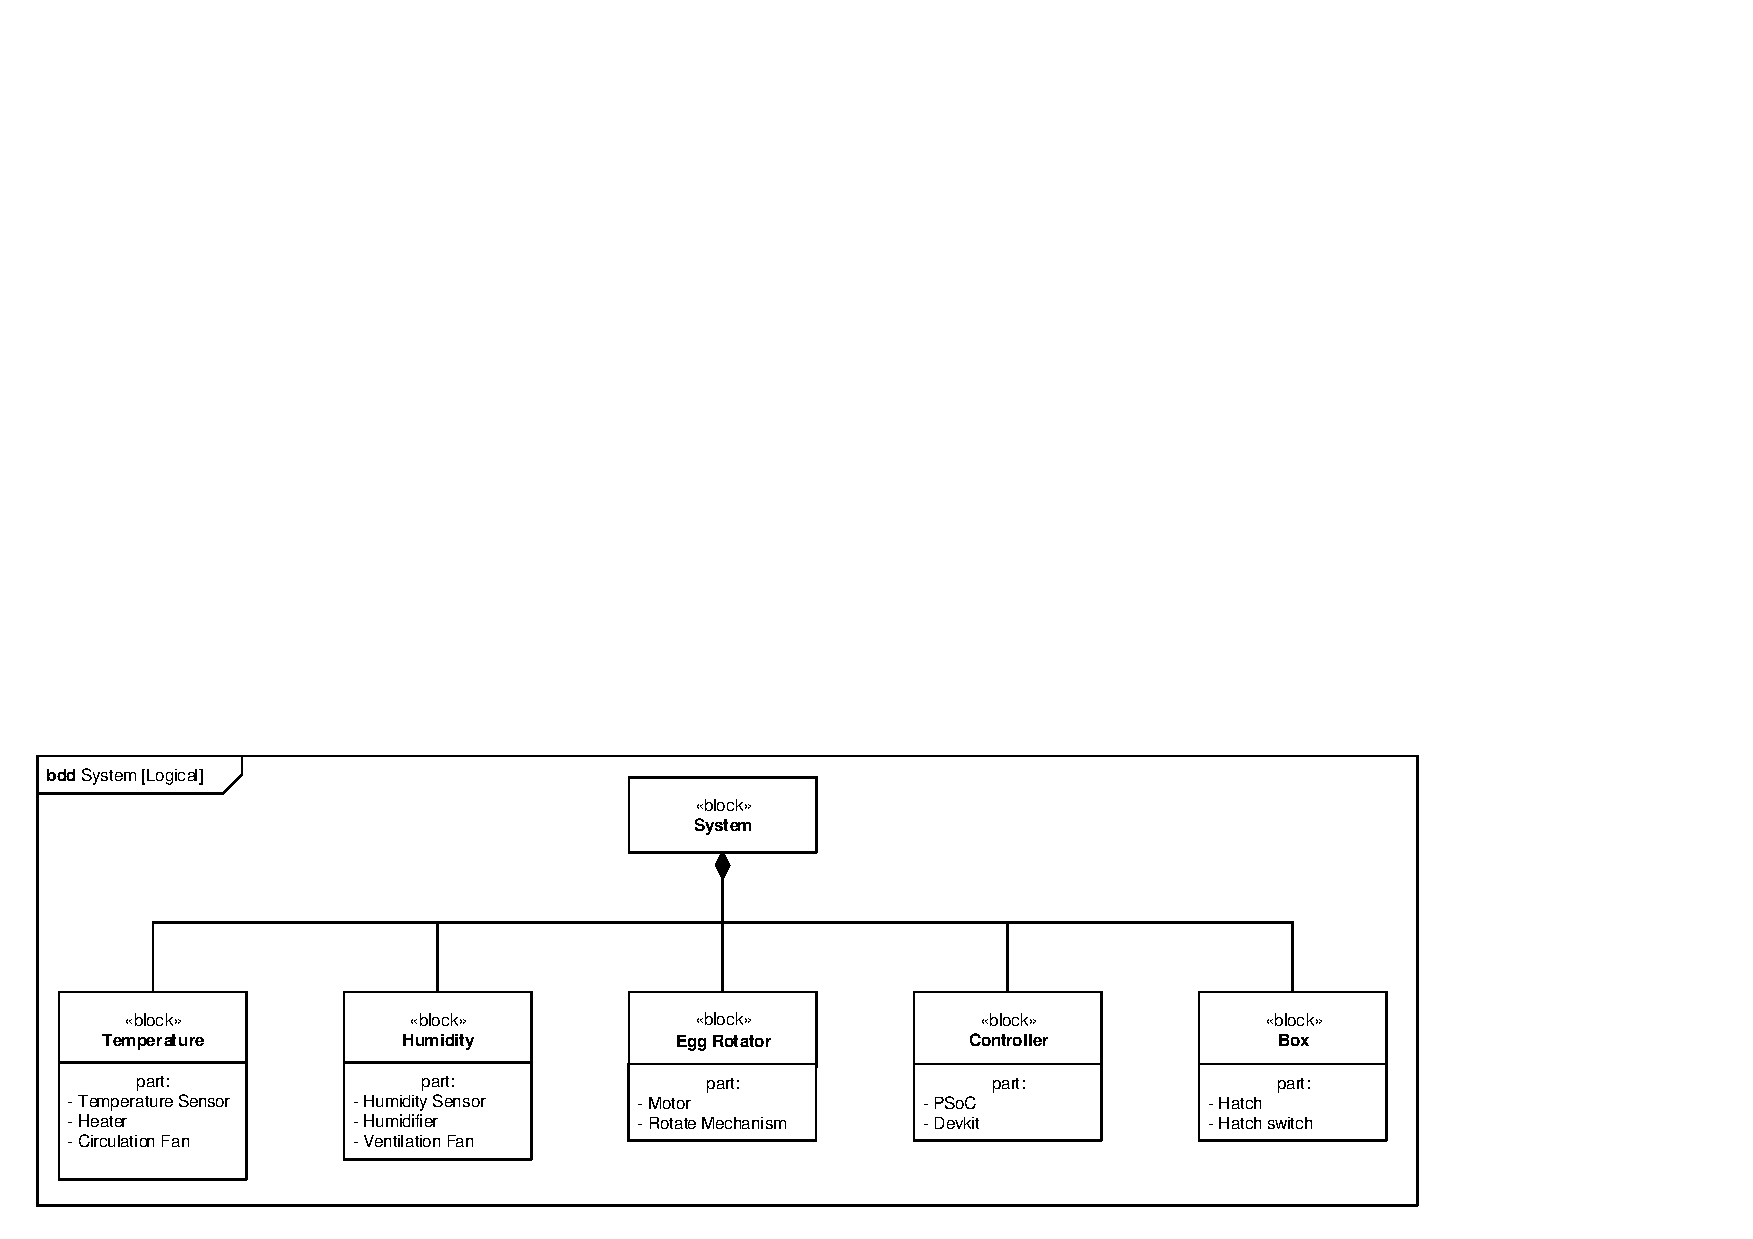
\includegraphics[width=\linewidth,page=1,trim=5mm 5mm 55mm 125mm]{./7_projektbeskrivelse/systemarkitektur/diagrammer/SYSML_Diagrammer_v4.pdf}
\caption[Diagram]{Logisk BDD for Systemet}
\label{fig:BDDLogisk}
\end{figure}
%scale=0.60,

Figur \ref{fig:BDDLogisk} viser de førnævnte dele samt nogle tilføjelser. For at opfylde krav om udluftning i Systemet er der blevet tilføjet en ventilations part under "Humidity" blokken, og for at nå en bedre varmefordeling er der ligeledes placeret en cirkulations part i "Heater" blokken.

"Box" blokken henviser til den fysiske rugekasse, der ikke er blevet lavet, og på samme måde henviser "Rotate Mechanism" parten i "Egg Rotator" blokken til den fysiske mekanisme, der fysisk skulle rotere emner i rugekassen.

Systemet blev herefter delt op i to fysiske dele: En Master del, som udgøres af DevKit8000 alene, samt en Slave del, der udgøres af PSoC3, samt de dele den kontrollerer. Der blev også taget stilling til hvordan de forskellige elementer skulle interagere med hinanden og igennem hvilket type interface. Dette er opsumeret i følgende fysiske BDD:

\begin{figure}[H]
\centering
\includegraphics[page=2,width=\linewidth,trim=5mm 5mm 210mm 20mm]{./7_projektbeskrivelse/systemarkitektur/diagrammer/SYSML_Diagrammer_v4.pdf}
\caption[Diagram]{Fysisk BDD for Systemet}
\label{fig:BDDFysisk}
\end{figure}

Som det fremgår af Figur \ref{fig:BDDFysisk}, blev det besluttet at kommunikation imellem de to blokke, PSoC3 og DevKit8000, skulle ske igennem SPI. Dette valg blev truffet ud fra foregående erfaringer med at kommunikere imellem disse igennem dette interface, opnået i forbindelse med andre opgaver. Som det også fremgår, blev det ligeledes besluttet, at alle sensorer skulle være digitale, og at de skulle være af I2C typen, da det ligeledes var noget vi havde erfaring med gennem tidligere opgaver.

Siden systemet grundlæggende udvikles til at skulle kunne håndtere forskellige typer af æg, der evt. har forskellige krav til omgivelsernes temperatur, blev det også valgt at den styrende udgang til varmeregulering skulle være af en velkendt, variabel type, og her faldt valget på et PWM signal.

For flere detaljer omkring de interne forbindelser henvises til IBD'erne i dokumentationen.
\clearpage
\subsection{Software Diagrammer}

Fra Use Casene blev den grundlæggende software arkitektur fastlagt ved brug af de sædvanlige metoder; domæne-modeller, sekvens- og klasse-diagrammer og state machines. 

På Figur \ref{fig:StateMachine} ses state machine diagrammet for systemet, som giver et overblik over opførelsen af systemet. 

\begin{figure}[H]
\centering
\includegraphics[page=3,scale=0.85,trim=5mm 5mm 230mm 190mm]{./7_projektbeskrivelse/systemarkitektur/diagrammer/ArkitekturDiagrammer.pdf}
\caption[Diagram]{State Machine for Systemet}
\label{fig:StateMachine}
\end{figure}

På Figur \ref{fig:KlasseDiagram} ses klassediagrammet, som viser de funktioner, der skal implementeres:

\begin{figure}[H]
\centering
\fbox{\includegraphics[page=4,scale=0.9,trim=5mm 5mm 100mm 230mm]{./7_projektbeskrivelse/systemarkitektur/diagrammer/ArkitekturDiagrammer.pdf}}
\caption[Diagram]{Klassediagram for Systemet}
\label{fig:KlasseDiagram}
\end{figure}

Det er værd at bemærke, at hovedparten af dette software afvikles på PSoC3.

For sekvensdiagrammerne henvises til dokumentationen.

\subsection{Hardware}
Følgende afsnit omhandel Designvalg og implementering af de 
\subsection{Hardware}
Følgende afsnit omhandel Designvalg og implementering af de 
\subsection{Hardware}
Følgende afsnit omhandel Designvalg og implementering af de 
\input{7_projektbeskrivelse/design_og_implementering/hardware.tex}
%rækkefølge
%Sensor
%regulerig
%stepmotor
%sekvens timer
%SPI protocol
%Main
%driver
%GUI

%\subsection{Sensor - Dannie} \label{Sensor}

\subsubsection{Design}

Til udrugningen skal luftfugtigheden og temperaturen holdes på et fast niveau. 
Ved lidt hurtigt søgning i lokal varekakaori, er der fundet en sensor som kunne måle begge dele. Sensoren har dog en kompliceret protokol. Efter noget research og forsøg med at få lavet et program, viser det sig dog, at for at få sensoren til at virke, vil det kræve en ekstra microprocessor kun til at arbejde med sensoren. Derfor vælges sensoren HIH6121-021, som har samme nødvendige funktionalitet som sensoren SHT71 dog knapt så fintfølende. Sensoren overholder stadigvæk kravspecifikationerne og kommunikerer med en standard I2C protokol, hvilket vil være forholdsvist nemt at implementere. HIH6121-021 sensoren har et spændingsniveau mellem \SI{2.3}{\volt} og \SI{5.5}{\volt}\cite{HIH61xx}, da PSoC3 spændingsniveau ligger på \SI{3.3}{\volt} eller \SI{5}{\volt} vil det ikke være et problem uanset PSoC3 spændingsniveau. Da sensoren følger en I2C protokol\cite{HIH61xx_I2C}, skal der ikke tages hensyn til støj.

\subsubsection{Implementering}

Der er implementeret 5 funktioner til HIH6121-021 softwaren:
\begin{enumerate}
\item \texttt{init\_HIH61xx()} har til formål at implementere I2C standardkomponentens kode i PSoC3 programmet. 

\item \texttt{measure\_HIH61xx()} har til formål at kommunikere med sensoren. Den får sensoren til at måle luftfugtighed og temperatur.

\item \texttt{read\_HIH61xx()} har til formål at aflæse de målte værdier fra sensoren. Den aflæser 4 data bytes, som funktionen allokerer og behandler lokalt. 

\item \texttt{getTemp()} har til formål at returnere den sidste aflæste temperaturværdi fra sensoren. 

\item \texttt{getHumid()} har til formål at returnere den sidste aflæste luftfugtighedsværdi fra sensoren.
\end{enumerate}

Funktionerne er delt op, således at hver enkelt modul som skal bruge data fra sensoren, ikke skal kommunikere hver gang de skal bruge data, de kan simpelt kalde \texttt{getTemp()} eller \texttt{getHumid()} og derved få de sidste opdaterede værdier. \texttt{measure\_HIH61xx} og \texttt{read\_HIH61xx} er lavet således at de kan blive kaldt når main programmet har tid til at opdatere værdierne af luftfugtighed og temperatur, så er det op til main programmet at bestemme hvor ofte værdierne skal opdateres. 

%
%\subsubsection{Design}
%Processen at udruge et æg tager op til flere uger, og det er vigtigt at kunne holde styr på de forskellige faser i udrugningen. Derfor er der brug for en timer, som over lang tid kan holde styr på tiden.
%
%Umiddelbart har vi tre muligheder på PSoC3-platformen, som opfylder ovenstående ønsker:
%
%1) En timer som periodisk genererer et interrupt, som kan bruges til at optælle en variabel.
%
%2) En count-down timer som udfører en handling, når timeren har talt ned. Timeren indstilles herefter til tiden indtil den næste handling skal udføres.
%
%3) En Real-Time Clock (RTC), hvor en alarm kan sættes til det næste tidspunkt hvorpå der skal ske en handling.
%
%Mulighed nr. 1 har fordelen at vi hele tiden har en variabel, som beskriver hvor lang tid der er gået - denne information kan bruges, når brugeren skal informeres om tiden.
%
%\subsubsection{Implementering}
%Implementeringen af timeren foregår i PSoC Creator, hvor der vælges en timerkomponent, en clock og en ISR (Interrupt Service Rutine). Clocken sættes til timerens clock-indgang, og ligeledes sættes ISR-komponenten til timerens interrupt-udgang.
%
%Timer og clock indstilles så interruptet fremkommer hvert minut.
%
%I softwaren, i ISR-funktionen, sættes et flag til "true" hver gang timeren genererer et interrupt. Dette flag tjekkes i main-løkken, hvorefter minuttælleren forøges med 1. 
\subsection{Regulering - Morten}

Regulering af luftfugtighed og temperatur er implementeret på stort set samme måde, så begge vil blive beskrevet i dette afsnit. Selve design og implementering er en kombination af PSoC3 hardwareblokke og software, til at styre disse hardwareblokke. Funktionerne dette afsnit omhandler, er funktionerne beskrevet under "Humidity" og "Temperature" i figur \ref{fig:KlasseDiagram}.

\textbf{Design}

Funktionerne til at styre reguleringen af temperatur og luftfugtighed er 

\begin{itemize}
\item \texttt{regTemp(float)}/\texttt{regHum(float)} - Skal starte reguleringen af hhv. temperatur og luftfugtighed
\item \texttt{stopTemp()}/\texttt{stopHum()} - Skal afbryde reguleringen
\item \texttt{pauseTemp()}/\texttt{pauseHum()} - Skal afbryde regulering når den kaldes, og igangsættes reguleringen når den kaldes igen
\end{itemize}

Det ønskes, at reguleringen skal foregå automatisk efter at være igangsat. Dertil benyttes timere til at, med faste mellemrum, generere interrupts, og reguleringen vil da foregå i Interrupt service rutinen. Da reguleringen ikke er noget der er tidskritisk vil disse ISR have lav prioritet.

Temperatur og luftfugtighed har forskellige forudsætninger, og det giver anledning til følgende designbeslutninger:
\begin{itemize}
\item Varmeudveksling med omgivelserne vil gøre, at systemets temperatur konstant vil falde og systemet skal derfor have tilført en bestemt mængde energi hele tiden. Da varmelegemet styres ved hjælp af et PWM signal, skal ISR'en udføre en PID regulering og output af denne skal bestemme Duty Cycle af PWM signalet. 
\item Under forudsætningen af at systemet er godt isoleret, vil luftfugtigheden ikke falde. Så snart temperaturen er stabil, vil luftfugtigheden også være stabil. Da øgningen af luftfugtighed foregår via åbning og lukning af en magnetventil, skal ISR'en blot vurdere om luftfugtigheden er for lav, og åbne for ventilen hvis den er.
\end{itemize}
Ydermere bemærkes det at
\begin{itemize}
\item Da systemet ikke underbygger en mulighed for aktivt at sænke luftfugtigheden, er det vigtigt, at reguleringen ikke tilføjer for store mængder fugtighed.
\item Da luftfugtigheden er afhængig af temperaturen er det vigtigt, at PID reguleringen ikke laver oversving, da dette kan resultere i for høj luftfugtighed.
\end{itemize}
\clearpage
Begge reguleringer kræver information vedrørende hhv. systemets aktuelle temperatur og luftfugtigheden, og til dette anvendes de funktionerne beskrevet i afsnittet \ref{Sensor} om sensoren.

Ligeledes laves der i ISR'erne, er en underrutine, der skal holde øje med stabiliteten af systemet ved at

\begin{itemize}
\item Monitorere hvorvidt systemet når de krævede niveauer indenfor den tilladte tid
\item Monitorere om systemet er stabilt og holder de krævede niveauer indenfor de tilladte grænser
\item Meddele brugeren hvis de to forrige punkter ikke overholdes
\end{itemize}

som er påkrævede funktionaliteter iht. kravspecifikationen.


\textbf{Implementering}

Alle \texttt{reg},\texttt{pause} og \texttt{stop} funktioner er implementeret ved hjælp af de standardfunktioner, der er tilknyttet de hardwareblokke, der blev benyttet til de forskellige formål; hver regulering havde sin egen timer blok og tilhørende funktioner, og temperaturreguleringen havde ligeledes en PWM blok, til styring af varmelegemet samt cirkulations-ventilatoren. Cirkulationsventilatorens duty-cycle sættes til en fast værdi.

Som eksempel på implementering af funktionerne vises \texttt{pauseHum()}:

\begin{figure}[H]
\centering
\fbox{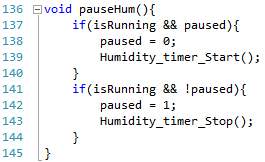
\includegraphics[scale=.80]{./7_projektbeskrivelse/design_og_implementering/software/billeder/pausehum.PNG}}
\caption[Diagram]{Implementering af \texttt{pauseHum()}}
\label{fig:PauseHum}
\end{figure}

Som det ses af Figur \ref{fig:PauseHum} benyttes funktionerne \texttt{Humidity\_timer\_Stop()} og \newline \texttt{Humidity\_timer\_Start()}, der starter og stopper for timeren, der skaber de interrupts, der foretager reguleringen af luftfugtigheden. De øvrige funktioner er implementeret på samme vis. Flagene \texttt{isRunning} og \texttt{paused} benyttes i rutinerne til at afgøre om ting startes, stoppes eller der ingenting skal foretages. Se kildekoden og dokumentation for flere detaljer ang. implementering af disse.

Selve reguleringen foregår ud fra differensen mellem de aktuelle og de ønskede værdier for temperatur og luftfugtighed; til regulering af luftfugtighed benyttes en simpel if-sætning, og til varmeregulering er implementeret følgende hjælpe-rutine:

\begin{figure}[H]
\centering
\fbox{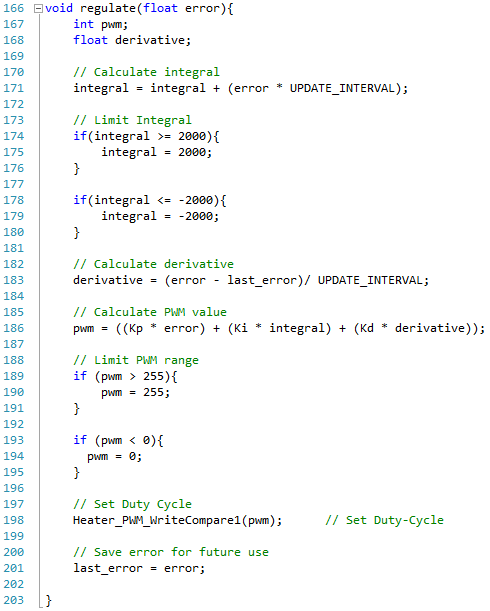
\includegraphics[scale=.80]{./7_projektbeskrivelse/design_og_implementering/software/billeder/pidroutine.PNG}}
\caption[Diagram]{PID hjælperutine}
\label{fig:PIDRutine}
\end{figure}

Som det ses af linie 198 anvendes igen standard funktioner.

Til at undersøge stabiliteten af systemet er implementeret en hjælpefunktion kaldet \texttt{stabilityControl(float)}. Den er opbygget af en kringlet mængde if-sætninger, flag og counters, så funktionaliteten kan bedst beskrives gennem dette flowchart:

\begin{figure}[H]
\centering
\fbox{\includegraphics[scale=0.8,page=5,trim=5mm 5mm 110mm 5mm]{./7_projektbeskrivelse/design_og_implementering/software/billeder/Varmeregulering.pdf}}
\caption[Diagram]{Flowdiagram for \texttt{stabilityControl(float)}}
\label{fig:stabilityControl}
\end{figure}

For mere information henvises til kildekoden.

\newpage
\subsection{Æggevending - Andreas}
Hele æggevendemekanismen indeholder 3 dele, disse er en fysisk stepmotor, en mekanisk vendeopsætning, samt en software styring af stepmotoren.
Den fysiske stepmotor er valgt som en unipolær, gearet stepmotor\footnote{Se datablad \cite{Stepmotor}}. Den mekaniske del er ikke implementeret, men der er foretaget designovervejelser over denne del, og software styringen er beskrevet i den følgende del af rapporten.

\subsubsection{Design}
Til stepmotorstyringen er der overvejet at lave med hensyn til stepping metode. De relevante metoder til dette projekt er enkelt faset full stepping, dobbelt faset full stepping, eller half stepping. Da kravene til motorens præcision er meget lave, så er half stepping, som har en højere opløsning, hurtigt sorteret fra. Valget der nu skal tages er mellem større moment eller lavere strømforbrug med evne til hurtigere hastighed. Her er der som udgangspunkt valgt at tage 2 faset stepping som har det højere moment.

Efter stepping metoden er på plads, så skal udførelsen af tidsintervallerne mellem hvert step overvejes. Her blev det bestemt at styringen ikke skulle være tidskritisk, og derfor blev denne lavet med et interrupt og en timer.

Æggene skal efter anbefalinger roteres en halv omgang ad gangen, og der skal ikke foretages hele omdrejninger, derfor skal der mellem hver halv-rotation ændres retning af motoren.

\subsubsection{Implementering}
Stepmotorstyringen blev som udgangspunkt designet og testet med den to-faset full step styring som var planlagt, men grundet en fejl der opstod i en afsluttende test, så blev en tidlig version som var lavet med enkelt faset full stepping brugt i stedet.
Antal steps der skulle tages for at en halv rotation af motoren endte op på 1024 stk.

Tidsintervallerne der blev testet med stepmotorstyringen blev sat til 1, 2 og 5ms, der opstod fejl ved 1ms intervallerne, mens der ingen var ved 2 og 5ms. Den senere test der lavede fejl opstod ved 2ms interval og der blev forhøjet til 2.73ms som var den umiddelbare maximum interval på den allerede indførte 16bit timer, dette var dog ikke nok, og en enkelt faset full step styring blev genbrugt.

Efter revideringen af motorstyringen opstod der ingen problemer og denne kunne også implementeres under den samlede integrationstest. Der er ikke taget hensyn til en evt. gearing af den mekaniske del af æggevendingen.

\subsection{Sekvenstimer - Simon og Stine}

\subsubsection{Design}
Processen at udruge et æg tager op til flere uger, og det er vigtigt at kunne holde styr på de forskellige faser i udrugningen. Derfor er der brug for en timer, som over lang tid kan holde styr på tiden.

Umiddelbart har vi tre muligheder på PSoC3-platformen, som opfylder ovenstående ønsker:

1) En timer som periodisk genererer et interrupt, som kan bruges til at optælle en variabel.

2) En count-down timer som udfører en handling, når timeren har talt ned. Timeren indstilles herefter til tiden indtil den næste handling skal udføres.

3) En Real-Time Clock (RTC), hvor en alarm kan sættes til det næste tidspunkt hvorpå der skal ske en handling.

Mulighed nr. 1 har fordelen, at vi hele tiden har en variabel, som beskriver hvor lang tid der er gået - denne information kan bruges, når brugeren skal informeres om tiden.

\subsubsection{Implementering}
Implementeringen af timeren foregår i PSoC Creator, hvor der vælges en timerkomponent, en clock og en ISR (Interrupt Service Rutine). Clocken sættes til timerens clock-indgang, og ligeledes sættes ISR-komponenten til timerens interrupt-udgang.

Timer og clock indstilles så interruptet fremkommer hvert minut.

I softwaren, i ISR-funktionen, sættes et flag til "true" hver gang timeren genererer et interrupt. Dette flag tjekkes i main-løkken, hvorefter minuttælleren forøges med 1. 

\newpage
\subsection{PSoC SPI - Simon og Stine}\label{psoc_spi}

\subsubsection{Design}
Der ønskes en kommunikation imellem PSoC3 og DevKit8000. Denne kommunikation skal foregå over SPI.
Formålet med kommunikationen er, at brugeren af rugemaskinen skal kunne bruge en brugergrænseflade på DevKittet til at kommunikere med PSoC3. Brugeren skal kunne starte og stoppe udrugningen samt kunne se en status af temperatur, luftfugtighed og tid på skærmen.

DevKittet kan sende følgende beskeder til PSoC3:
\begin{itemize}
  \item En start kommando - Starter udrugningssekvensen. Starter timer, sætter temperatur og luftfugtighed. 
  \item En slut kommando - Stopper udrugningssekvensen. Stopper timer, temperatur og luftfugtighed.
  \item En status kommando for temperatur - Send status på temperatur.
  \item En status kommando for luftfugtighed - Send status på luftfugtighed.
  \item En status kommando for tid - Send den forløbne tid.
\end{itemize}

En protokol for SPI bliver udarbejdet for at sikre, at DevKit8000 og PSoC3 sender og modtager det samme.
Det besluttes, at der sendes 16 bit ad gangen. Af disse 16 bit er de 4 første reserveret til adressen, de næste 4 til kommandoen og de sidste 8 til data.
Start/Slut beskeden får samme adresse, men hver sin kommando.
Status beskederne for temp, luftfugtighed og tid får hver sin adresse, men samme kommando.
Adresserne og kommandoerne er blevet valgt som følgende:

Adresser er markeret med \textcolor{red}{rød} og kommandoer er markeret med \textcolor{green}{grøn}.

\begin{table}[H]
    \begin{tabular}{|c|c|c|}
        \hline
        \textbf{Beskrivelse}&\textbf{Bitmønster}\\\hline
        Start og Slut&\textcolor{red}{0001}|\textcolor{green}{0001} og \textcolor{green}{0010}\\\hline
        Temperatur&\textcolor{red}{0010}|\textcolor{green}{0011}\\\hline
        Luftfugtighed&\textcolor{red}{0011}|\textcolor{green}{0011}\\\hline
        Tid&\textcolor{red}{0100}|\textcolor{green}{0011}\\\hline
    \end{tabular}
    \caption[Tabel]{Adresse og kommando bitmønster\hfill \textcolor{white}{.}}
    \label{tab:addrcmd}
\end{table}

\subsubsection{Implementering}

SPI kommunikationen blev implementeret i en interrupt service rutine, der står for dekodningen af data fra SPI.
Implementeringen betod i at oprette en switch case, der skifter på adressen sendt fra DevKit8000.
Inde i switch case'en blev der også tilføjet en if-sætning for at kunne skifte imellem Start kommandoen og Slut kommandoen, idet disse deler adresse.
\clearpage
Hvis kommandoen \textcolor{green}{Start} registreres skal der ske følgende:
\begin{itemize}
  \item Sæt temperatur til den ønskede temperatur på 37 grader.
  \item Sæt luftfugtighed til den ønskede luftfugtighed på 45.
  \item Nulstil tiden, countInMinutes.
  \item Start timeren.
\end{itemize}

Hvis \textcolor{green}{Slut} kommandoen derimod registeres skal følgende ske:
\begin{itemize}
  \item Stop regulering af temperatur.
  \item Stop regulering af luftfugtighed.
  \item Stop timeren.
\end{itemize}

Implementeringen af status på temperatur, luftfugtighed og tid er ens, men varierer
i form af det der bliver sendt tilbage til DevKit8000. 
For at sende data til Devkittet skal der sendes en SPI besked. Denne besked indeholder data, indsamlet fra sensoren. 

Implementeringen for afsendelsen af data ses nedenfor, hvor der bliver sendt en temperatur.
\begin{lstlisting}
/*Switch case (addr)*/
/*Send status case in switch case*/
case 0x2: //status temperature
			if (cmd == 0x3) //command status
            {   
                //clear buffer before sending
                SPIS_1_ClearTxBuffer(); 
                //send data temp from sensor to devkit
                SPIS_1_WriteTxData(getTemp());
            }
			break;
\end{lstlisting}

Som det ses på koden er det adressen 0x2 der svarer til temperatur. Herefter skal kommandoen checkes. Kommandoen for 'Status' er 0x3, som nævnt i design afsnittet.
For at sende temperatur data'en benyttes SPI-kommandoen for at skrive data. Parameteren der skal sendes er i dette tilfælde, \texttt{getTemp()}. Denne parameter stammer fra sensoren, og indeholder den temperatur, der skal vises på DevKittet.

\newpage
\subsection{PSoC main - Simon og Stine}

\subsubsection{Design}

For at forenkle implementeringen af udrugningssekvenser er det blevet besluttet
at starte med kun at implementere forløbet for en enkel ægtype. 
Følgende forløb ønskes:

\begin{itemize}
  \item Tiden nulstilles når udrugningssekvensen påbegyndes.
  \item Temperaturen sættes til 37 grader og luftfugtigheden sættes til 45.
  \item Hver 12. time skal æggene vendes.
  \item Hvert døgn skal det simuleres at hønen forlader æggene i 30 minutter. Dette gøres ved at sætte temperaturen ned til 20 i 30 minutter.
  \item Efter 18 dage skal luftfugtigheden sættes op til 75.
  \item Efter 21 dage er udrugningssekvensen slut. Timeren skal stoppes og DevKit8000 informeres.
\end{itemize}
Forløbet for udrugningssekvensen er inspireret fra hjemmesiden\footnote{Hønsehuset.dk \cite{Rugetips}}.

Forløbet ønskes implementeret som en for-løkke, der bliver kørt igennem en gang i minuttet.
Der skal tages hensyn til de tidsbegænsninger der er i udrugningssekvensen, f.eks. 12 timer og 18 dage.
For at håndtere dette, vælges det at omregne tiden til minutter, hvorefter man vha. if-sætninger, kan håndtere begrænsningerne.

Tidsbegrænsningerne omregnet til minutter:
\begin{itemize}
  \item 12 timer = 720 minutter.
  \item 24 timer = 1440 minutter.
  \item 18 dage = 25920 minutter.
  \item 21 dage = 30240 minutter.
\end{itemize}


\subsubsection{Implementering}
Implementeringen af forløbet for udrugningen blev lavet i et PSoC projekt.

Operatoren modulus blev valgt til at hjælpe med at implementere de tidsbegrænsede dele af forløbet.
En variabel countInMinutes blev oprettet til at indeholde tiden gået siden start.
Da countInMinutes indeholder tiden der er gået, kan modulus bruges til at overholde tidsbegrænsningerne.
Eksempel på brug af modulus: 

\texttt{if(countInMinutes \% 720 == 0)}

Denne if-sætning checker på, om det er tid til æggevending, hvilket er hvert 720. minut.

For hver af punkterne i forløbet (se design afsnit) blev der oprettet en if-sætning, magen til den ovenfor.
Ud over if-sætningerne for 12 timer, 24 timer, 18 dage og 21 dage skulle der oprettes en if-sætning til at håndtere simuleringen 
af at hønen forlader reden. 
Hver 24 time bliver temperaturen sat til en lavere temperatur og den samtidige tid, countInMinutes, bliver gemt i en variabel timeStamp.
Derudover bliver et flag sat.
Dette flag samt timeStamp benyttes i en if-sætning der sørger for at temperaturen kun er sænket i 30 minutter. 

\subsection{Devkit driver - Mathias}
\subsubsection{Design}

Da Devkit8000 er et embedded system, med et Linux baseret OS, skal der for at tilgå fysiske resourcer benyttes et driverlag. 

Driveren der skrives til Devkit8000 har brug for følgende funktionalitet:

\begin{itemize}
  \item Skal kunne kommunikere over SPI protocol til PSoC3.
  \item Skal kunne modtage interrupt fra lågen.
\end{itemize}

Til SPI Driveren er der allerede udarbejdet et skelet i faget I3HAL, hvor der er lavet en driver, som kan kommunikere over SPI\footnote{Redmine Driver \cite{redmine_driver}}. Der tages udgangspunkt i denne, der ønskes dog tilføjet følgende funktionalitet:

\begin{itemize}
  \item Tilpasning til den tidligere definerede protocol i projektet, se afsnit \ref{psoc_spi}.
  \item Automatisk oprettelse af node filer ved at tilføje oprettelse af \texttt{driver class} og \texttt{driver device}.
  \item Tilføjelse af en interrupt line, GPIO samt ISR til interrupt linen. 
  \item Der skal ændres i read funktionen (funktionen der bruges til at tilgå driveren) så den kan bruges til både SPI og interrupt.
\end{itemize}

Designmæssigt vælges det at begge funktionaliteter samles i en driver frem for at splitte det op i to forskellige drivere. Dette vælges, da det ikke anses for nødvendigt, at de to drivere skal kunne benyttes uafhængigt af hinanden.

\subsubsection{Implementering}

For at oprette node filerne automatisk, som er applikationers tilgang til driver, tilføjes objekter af typen \texttt{device} og \texttt{class}. Der oprettes en enkelt \texttt{device} class, samt et device for hver fil der skal oprettes. For at tilpasse driveren til den ønskede SPI protocol oprettes tre "read" filer til at hente "Temp", "Humid"  og "Time"  samt en read fil til interrupt linien. Til SPI delen oprettes ligeledes en SPI "write". 

%Følgende kode blev derfor tilføjet til driveren init funktion:
%\begin{lstlisting}
%//Declare device and class
%static struct device* psoc_device[MINOR_NUM];
%static struct class* psoc_class;
%
%//In init function
%//Create class
%psoc_class = class_create(THIS_MODULE, "psoc3");
%
%//create devices (acces files)
%for ( i = 0; i < MINOR_NUM-1; i++)
%		psoc_device[i] = device_create(psoc_class, NULL, MK_DEVNO, 
%				NULL, "psoc%d", i);
%interrupt_device = device_create(psoc_class, NULL, MKDEV(MAJOR(devno),4), 
%				NULL, "psoc_interrupt%d",0); 
%\end{lstlisting}
%
%MK\_DEVNO tildeler filen det rigtige minor number, som senere benyttes til at retunere de rigtige værdier når der læses fra filen.

Ligeledes blev der i \texttt{exit} funktionen tilføjet kode til at rydde op igen.

For at kunne styre hvilke filer, der blev brugt til at tilgå hvad, blev der i \texttt{read} og \texttt{write} funktionerne lavet en "Switch case", som kigger på driverens minor nummer (filen der bliver tilgået).
%, ex på dette kan ses i koden for read funktionen:
%
%\begin{lstlisting}
%//Read funktion
%minor = MINOR(filep->f_dentry->d_inode->i_rdev);
%	switch (minor)
%	{
%		case 1:	
%			if(psoc_spi_read_reg16(0x02,&result) < 0)
%				return -1; 
%			break;
%		case 2:	
%			if(psoc_spi_read_reg16(0x03,&result) < 0)
%				return -1; 
%			break;
%		case 3:	
%			if(psoc_spi_read_reg16(0x04,&result) < 0)
%				return -1; 
%			break;
%		case 4:
%			wait_event_interruptible(interruptlineQ, (flag == 1));
%			result = gpio_get_value(GPIO_KEY);
%			flag = 0;
%			break;en man henvender sig til, giver den data man ønsker. Når man henvender sig til filen som giver minor number 4, ender man i \newline\texttt{wait\_event\_interruptible(interruptlineQ, (flag == 1))}. Funktionen er kombineret med en interrupt service rutine, som sætter \texttt{flag} til at være lig 1, samt sender et \texttt{wake\_interruptible}. Dette sikrer at der kun kan læses data når der bliver registreret en ændring på rising eller falling edge.

Der blev desuden lavet et script, for at insætte driveren, hotplug modulet, samt ændre indstillinger på den allerede eksisterende cpld driver.
%
%\begin{lstlisting}
%insmod psocmod.ko
%insmod hotplug\_psoc\_spi\_device.ko
%
%echo 0x3 > /sys/class/cplddrv/cpld/spi\_route\_reg
%echo 0x1 > /sys/class/cplddrv/cpld/ext\_serial\_if\_route\_reg
%\end{lstlisting}

\subsection{Devkit GUI - Mathias}

\subsubsection{Design}

Til den grafiske burgerflade ønskes der et meget simpelt design. Den grafiske brugerflade skal have følgende funktionaliteter:

\begin{itemize}
	\item Skal kunne starte og stoppe for udrugningssekvensenn, 
	\item Skal kunne vise den forløbne tid, samt den aktuelle temperatur og luftfugtighed.
	\item Skal give besked til brugeren, når lågen er åben.
\end{itemize}

Dette giver et basisudkast at arbejde ud fra til implementeringsfasen.

\subsubsection{Implementering}
Til at lave GUI applikationen blev der anvendt Qt frameworket. Dette blev valgt, da det er et relativt simpelt framework at benytte. Det er baseret på C++.

Idet implementeringen af GUI applikationen samtidigt var en del af læringsprocessen i Qt, blev implementeringen meget metodisk. 

For at give et godt udgangspunk at arbejde ud fra, blev den grafiske del af programmet først implementeret. Det endelige grafiske design, implementeret i Qt, kan ses på figur \ref{fig:GUI}.

\begin{figure}[H]
\centering
\fbox{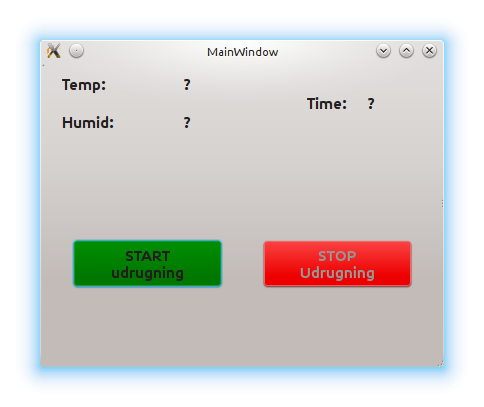
\includegraphics[page=1,width=((\linewidth)/10)*8]{./7_projektbeskrivelse/design_og_implementering/software/billeder/GUI.png}}
\caption[Figur]{GUI designet, implementeret i Qt.}
\label{fig:GUI}
\end{figure}

I designfasen blev den grafiske del holdt meget simpelt for at gøre det simpelt at implementere. Der blev derfor hurtigt lagt vægt på at få implementeret den underliggende software til applikationen.

 Der blev derfor udarbejdet et UML klassediagram for at give et overblik over de forskellige klasser, der skulle laves, deres relationer, samt nedarvningshierarki. Ligeledes blev det brugt til at give overblik over de forskellige metoder, der skulle laves under de forskellige klasser:

\begin{figure}[H]
\centering
\fbox{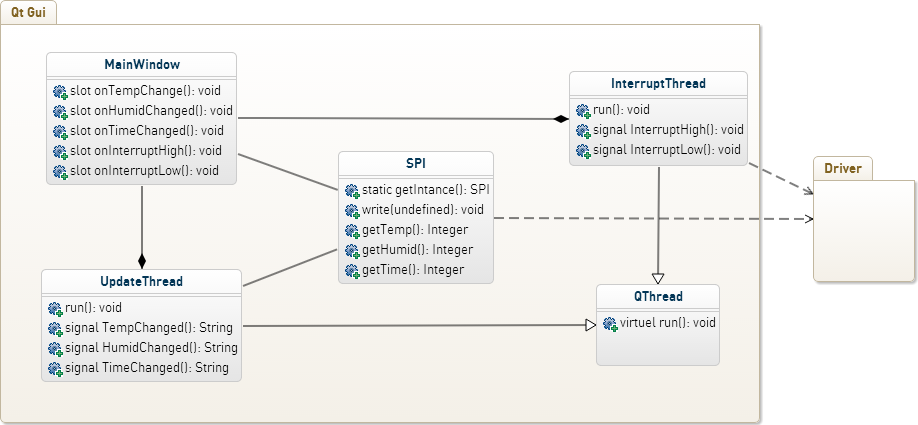
\includegraphics[page=1,width=\linewidth]{./7_projektbeskrivelse/design_og_implementering/software/billeder/klasse_diagram.png}}
\caption[Figur]{Klasse diagram over GUI applikationen.}
\label{fig:klasse_diagram}
\end{figure}

For at lave en grafisk applikation, som fungerer så flydende som muligt, blev der anvendt flertrådet programmering. Det blev valgt, at der blev benyttet en "main" tråd til at håndtere selve den grafiske, eventorienterede programmeringsdel. Der blev dertil lavet to datatråde, som hver især står for at skulle håndtere data og sende til "main" tråden. De to tråde blev lavet som klasserne UpdateThread og InterruptThread og blev, ud fra Qt dokumentationen omkring flertrådet programmering, lavet som nedarvninger fra klassen Qthread \footnote{Se Starting Threads with QThread\cite{Qthread}}.


\textbf{MainWindow:}
\texttt{MainWindow} er klassen, der står for at håndtere selve "main" vinduet. Klassen har nogle metoder, der håndterer de to trykknapper samt nogle forskellige slots. De forskellige slots anvendes til at fange signaler emittet fra de to andre tråde. 

\texttt{MainWindow} står for at oprette de to datatråde \texttt{InterruptThread} og \texttt{UpdateThread} og har kendskab til SPI klassen.

\textbf{SPI:}
SPI klassen er en klasse, der er tilpasset til at tage sig af kommunikationen til PSoC3 via den udarbejde driver. SPI klassen opretter derfor tre C++ file streams til at gå ud og læse på de tre driver nodes med temperatur, luftfugtighed og tid. Til at håndtere skrivningen over SPI kommunikationen blev der anvendt et C file handle. Dette blev anvendt frem for C++ fil behandlingen, da der er større kontrol over buffere, når der anvendes almindelig C. Da der er flere tråde, der skal kunne anvende SPI klassen, blev den givet en mutex, som den i hver af \texttt{get} og \texttt{write} metoderne låser i starten og frigives i slutningen. For at sikre at trådsynkroniseringen bliver holdt, er det nødvendigt, at der kun benyttes en fælles instans af klassen af de andre klasser. Det blev gjort via metoden \texttt{getInstance}, samt en privat constructor. SPI klassen kan derfor kun tilgås via metoden \texttt{getInstance}:

\begin{lstlisting}
SPI& SPI::getInstance()
{
    static SPI spi;
    return spi;
}
\end{lstlisting}

Idet metoden er erklæret static, kan metoden tilgås, selvom der ikke er oprette en instans af klassen. Første gang metoden så kaldes, opretter den en static instans af SPI klassen, som den så returnerer en reference dertil. Dette sikrer, at når metoden kaldes næste gang, er instansen allerede oprettet.

\textbf{UpdataThread:}
Klassen \texttt{UpdataThread} bruges til at gå ud og hente temperatur, luftfugtighed og tid, via SPI klassen. \texttt{UpdateThread} står herefter for at lave de hentede integer værdier om til Qstrings, med det ønskede formatering, og emitte de forskellige signaler til \texttt{MainWindow}, som så viser data'en.

\textbf{InterruptThread:}
\texttt{InterruptThread} står for at læse på interrupt linien i driveren. \texttt{InterruptThread} emmitter så et signal alt efter hvilken værdi der læses fra driveren. Hvis der sendes en \texttt{interruptHigh}, vises der en \texttt{Qmessagebox}, der informerer brugeren om, at lågen er åben. \texttt{InterruptLow} står så for at lukke denne \texttt{Qmessagebox} igen. 
\chapter{Accepttest}
Da vi ikke formåede at sammensætte og teste systemet i dets helhed, kan vi ikke godkende nedenstående accepttests. Vi har dog gennemført og godkendt flere af testene i et "subset" af systemet, som inkluderede sammensatte moduler.

\section{Accepttest for Use Case \usecaseref{Begynd udrugning}} 

%************************ Use Case 1 **************************************
 
 \subsection{Hovedscenarie}
\begin{center}

	\begin{tabular}{| p{3cm} | p{3cm} | p{3cm} | p{3cm} |}
		\hline
		Krav & Udførelse & Forventet resultat & Resultat \\ \hline
		% % % % % % % % % % % % % % % % % % % % % % % % % % % % 
		
		\multirow{2}{3cm}{Ved lågens åbning låses UI. Det forbliver låst indtil lågen lukkes.} 
		& Maskinen står i idle tilstand og lågen åbnes
		& UI låser
		& \\ \cline{2-4}
		
		&Lågen lukkes igen
		
		&UI låser op
		& \\ \hline 
		

	\end{tabular}
\end{center}

%\subsubsection{Undtagelser}
%\begin{center} 
%	\begin{tabular}{| p{3cm} | p{3cm} | p{3cm} | p{3cm} |}
%	\end{tabular}
%\end{center}

\section{Accepttest for Use Case \usecaseref{Udrug aeg}} 

%************************ Use Case 2 **************************************
 
 \subsection{Hovedscenarie}
\begin{center}

	\begin{longtable}{| p{3cm} | p{3cm} | p{3cm} | p{3cm} |}
		\hline
		Krav & Udførelse & Forventet resultat & Resultat \\ \hline
		% % % % % % % % % % % % % % % % % % % % % % % % % % % % 
		
		
		Systemet skal kunne regulere og holde en temperatur indenfor grænserne angivet i ikke funktionelle krav.
		&Systemet opstilles i omgivelser der ligger indenfor de påkrævede rammer. Systemet indstilles til at skulle holde 37$^\circ$C. Systemet sættes i gang og temperaturen aflæses efter 10 minutter. 
		&Maskinen kan regulere og holde temperaturen indenfor de angivne rammer. 
		& \\ \hline
		
		Systemet skal kunne regulere og holde en luftfugtighed indenfor grænserne angivet i ikke funktionelle krav.
		&Systemet opstilles i omgivelser der ligger indenfor de påkrævede rammer. Systemet indstilles til at skulle holde 70\% relativ luftfugtighed. Systemet sættes i gang og luftfugtigheden aflæses efter 10 minutter.
		&Maskinen kan regulere og holde luftfugtigheden indenfor de angivne rammer.
		& \\ \hline
		
		Maskinen kan vende æg med et bestemt interval. Æggene roteres indenfor de i ikke funktionelle krav specificerede grænser.
		&Æg-type specificeres, og systemet indstilles til at skulle vende æggene hvert 5. minut i en periode på 30 minutter. Æggenes vertikale akse markeres med en pil, der peger op. Systemet sættes i gang og kører i 30 minutter. Ved hver vending måles rotation af hvert æg, og deres rotation noteres. Efter hver rotation vendes hvert æg manuelt så orienteringsindikatoren (pilen) peger opad. 
		&Maskinen roterer alle æg indenfor den angivne grænse.
		& \\ \hline		
		
		Systemet skal ved afsluttet udrugning informere brugeren om dette.
		&Maskine indstilles til et 5 minutters udrugningsprogram og igangsættes. Det observeres at systemet informerer brugeren når sekvensen afsluttes.
		&Maskinen vil ved testsekvensens afslutning informere brugeren.
		& \\ \hline

		
		
	\end{longtable}
\end{center}
\subsection{Undtagelser}
\begin{center}

	\begin{longtable}{| p{3cm} | p{3cm} | p{3cm} | p{3cm} |}
	\hline
			Krav & Handling & Forventet resultat & Resultat \\ \hline
			% % % % % % % % % % % % % % % % % % % % % % % % % % % % 
			
			\multirow{2}{\linewidth}{Ved lågens åbning låses UI og udrugningssekvensens afbrydes midlertidigt. UI forbliver låst indtil lågen lukkes. Når lågen lukkes genoptages udrugnings- sekvensen.} 
			& Maskinen står I udrug-tilstand og lågen åbnes. \newline
			& UI låser og udrugningssekvensen stoppes.
			& \vspace{2.5cm} \\ \cline{2-4}
			
			&Lågen lukkes igen.
			
			&UI låser op og udrygningssekvensen genoptages.
			& \vspace{2.5cm} \\ \hline 
			
			Hvis det ikke er muligt at overholde temperaturen skal systemet informere brugeren.
			&Maskine opstilles i et lokale med temperatur indenfor de angivne grænser for opstilningsmiljø. Systemet indstilles til at skulle holde temperaturen på 40$^\circ$C, varmelegemet frakobles, og systemet aktiveres. \newline
			&Maskinen informerer brugeren. 
			& \\ \hline
			
			Hvis det ikke er muligt at overholde luftfugtigheden skal systemet informere brugeren.
			
			&Maskine opstilles i et lokale med luftfugtighed indenfor de angivne grænser for opstilningsmiljø. Systemet indstilles til at skulle holde luftfugtigheden på 70\% relativ luftfugtighed, luftfugtighedsreguleringsmekanismen  frakobles, og systemet aktiveres.
			
			&Maskinen informerer brugeren.
			
			& \\ \hline
					
			
		\end{longtable}
	\end{center}
\bibliography{../references/referencer}{}
% mappen bilag er tænkt til filer som ikke indgår i dok. men lavet i tilfælge af der bliver brug for den.
%\input{6_bilag/bilag}

%Generer en liste over opgaver der mangler at blive udført
%\listoffixmes

\end{document}
